% 2022-01-31 revised by Banbara
\documentclass[dvipdfmx]{beamer}

%\usepackage{bxdpx-beamer}% dvipdfmxなので必要
\usepackage{listings,jlisting} %ソースコード貼り付けのため
\usepackage{tikz}
\usetikzlibrary{positioning}
\usetikzlibrary{shadows}
%\AtBeginDvi{\special{pdf:tounicode 90ms-RKSJ-UCS2}} % しおりが文字化けしないように

\usepackage[deluxe]{otf}%hgt(太い明朝,ゴシック)を使うためのdeluxe
\usepackage{txfonts} % 数式・英文ローマン体を Lxfont にする
\renewcommand{\kanjifamilydefault}{\gtdefault}
\usepackage{graphicx,xcolor} % 文字の色

\usetheme{Warsaw}
%\usetheme{Darmstadt}
\setbeamertemplate{navigation symbols}{} % 右下のアイコンを消す
\setbeamertemplate{footline}[frame number] % スライド下のバーを消してフレーム番号を表示
\useoutertheme{shadow}                 % 箱に影をつける
\usefonttheme{professionalfonts}       % 数式の文字を通常の LaTeX と同じにする

%%%%%%%%%%%%%%%%%%%%%%%%%%%%%%%%%%%%%%%%%%%%%%%%%%%%%%%%%%%%%%%%
% User-defined Macro
%%%%%%%%%%%%%%%%%%%%%%%%%%%%%%%%%%%%%%%%%%%%%%%%%%%%%%%%%%%%%%%%
\newcommand{\compress}{\itemsep0pt\parsep0pt\parskip0pt\partopsep0pt}
% \newcommand{\compress}{\itemsep1pt plus1pt\parsep0pt\parskip0pt}
% \newcommand{\code}[1]{\lstinline[basicstyle=\ttfamily]{#1}}
\newcommand{\gringo}{\textit{gringo}}
\newcommand{\clasp}{\textit{clasp}}
\newcommand{\clingo}{\textit{clingo}}
\newcommand{\teaspoon}{\textit{teaspoon}}
\newcommand{\sat}{\textsf{SAT}}
\newcommand{\unsat}{\textsf{UNSAT}}
% \newcommand{\web}[2]{\href{#1}{#2\ \raisebox{-0.15ex}{\beamergotobutton{Web}}}}
% \newcommand{\doi}[2]{\href{#1}{#2\ \raisebox{-0.15ex}{\beamergotobutton{DOI}}}}
% \newcommand{\weblink}[1]{\web{#1}{#1}}
% \newcommand{\imp}{\mathrel{\Rightarrow}}
% \newcommand{\Iff}{\mathrel{\Leftrightarrow}}
% \newcommand{\mybox}[1]{\fbox{\rule[.2cm]{0cm}{0cm}\mbox{${#1}$}}}
% \newcommand{\mycbox}[2]{\tikz[baseline]\node[fill=#1!10,anchor=base,rounded corners=2pt] () {#2};}
% \newcommand{\naf}[1]{\ensuremath{{\sim\!\!{#1}}}}
% \newcommand{\head}[1]{\ensuremath{\mathit{head}(#1)}}
% \newcommand{\body}[1]{\ensuremath{\mathit{body}(#1)}}
% \newcommand{\atom}[1]{\ensuremath{\mathit{atom}(#1)}}
% \newcommand{\poslits}[1]{\ensuremath{{#1}^+}}
% \newcommand{\neglits}[1]{\ensuremath{{#1}^-}}
% \newcommand{\pbody}[1]{\poslits{\body{#1}}}
% \newcommand{\nbody}[1]{\neglits{\body{#1}}}
% \newcommand{\Cn}[1]{\ensuremath{\mathit{Cn}(#1)}}
% \newcommand{\reduct}[2]{\ensuremath{#1^{#2}}}
% \newcommand{\OK}{\mbox{\textcolor{green}{\Pisymbol{pzd}{52}}}}
% \newcommand{\KO}{\mbox{\textcolor{red}{\Pisymbol{pzd}{56}}}}
% \newcommand{\code}[1]{\lstinline[basicstyle=\ttfamily]{#1}}
% \newcommand{\lw}[1]{\smash{\lower2.ex\hbox{#1}}}
\newcommand{\llw}[1]{\smash{\lower3.ex\hbox{#1}}}

\newenvironment{tableC}{%
  \scriptsize
  \renewcommand{\arraystretch}{0.9}
  \tabcolsep = 0.6mm
  % \begin{tabular}[t]{p{6mm}|rlr|rlr|rlr|rlr|rlr}\hline
  %   \multicolumn{1}{l|}{\llw{問題   }} &
  \begin{tabular}[t]{l|rlr|rlr|rlr|rlr|rlr}\hline
    \multicolumn{1}{l|}{\llw{問題}} &
    \multicolumn{3}{c|}{UD1} &
    \multicolumn{3}{c|}{UD2} &
    \multicolumn{3}{c|}{UD3} &
    \multicolumn{3}{c|}{UD4} &
    \multicolumn{3}{c}{UD5} \\
    & 
    \multicolumn{1}{c}{既知の} & & \multicolumn{1}{c|}{ASP} & 
    \multicolumn{1}{c}{既知の} & & \multicolumn{1}{c|}{ASP} & 
    \multicolumn{1}{c}{既知の} & & \multicolumn{1}{c|}{ASP} & 
    \multicolumn{1}{c}{既知の} & & \multicolumn{1}{c|}{ASP} & 
    \multicolumn{1}{c}{既知の} & & \multicolumn{1}{c}{ASP} \\
    & 
    ベスト & &  & 
    ベスト & &  & 
    ベスト & &  & 
    ベスト & &  & 
    ベスト & &  \\
    \hline
  }{%
    \hline
  \end{tabular}
}
 % 自分用のマクロ

\title{解集合プログラミングを用いた\\ハミルトン閉路問題の解法}
\author{平手 貴大}
\date{2022年2月16日\\前期課程中間発表}
\institute{番原研究室}

\begin{document}
%%%%%%%%%%%%%%%%%%%%%%%%%%%%%%%%%%%%%%%%%%%%%%%%%%%%%%%%%%%%%%%%%%%
\frame{\maketitle}
%%%%%%%%%%%%%%%%%%%%%%%%%%%%%%%%%%%%%%%%%%%%%%%%%%%%%%%%%%%%%%%%%%%
\begin{frame}{ハミルトン閉路問題(Hamiltonian Cycle Problem; HCP)}
  \begin{itemize}
  \item \alert{ハミルトン閉路問題}
    \begin{itemize}
    \item 与えられたグラフの全頂点をちょうど一度ずつ
      通る閉路が存在するかどうかを判定する問題である.
    \item 始点と終点が一致するという閉路の条件を
      取り除けば,ハミルトン路問題となる.
    \end{itemize}
  \item \alert{最短ハミルトン閉路問題}
    \begin{itemize}
    \item グラフの辺に距離が付随しているときに,
      最短距離のハミルトン閉路を求める問題である.
    \end{itemize}
  \item \alert{コスト制約付きハミルトン閉路問題}
    \begin{itemize}
    \item ハミルトン閉路問題に,距離の総和が所与の閾値以下
      (または以上)であることを制約条件として付加した問題である.
    \item 最近,二分決定グラフを用いた解の高速列挙アルゴリズムが提案されている~[湊+, 2020].
    \end{itemize}
  \end{itemize}
  \begin{alertblock}{}
    本研究では,無向グラフ上のハミルトン閉路問題
    およびその関連問題を対象とする.    
  \end{alertblock}
\end{frame}

%%%%%%%%%%%%%%%%%%%%%%%%%%%%%%%%%%%%%%%%%%%%%%%%%%%%%%%%%%%%%%%%%%%
\begin{frame}{解集合プログラミング(Answer Set Programming; ASP)}

  \begin{itemize}
  \item \alert{ASP 言語}は,一階論理に基づく知識表現言語の一種.
  \item \alert{ASP システム}は,論理プログラムから
    安定モデル意味論~{\scriptsize[Gelfond and Lifschitz, '88]}
    に基づく解集合を計算するシステム.
  \item 近年,SAT 技術を応用した高速 ASP システムが開発され,
    スケジューリング,プランニング,システム生物学,システム検証
    など様々な分野への実用的応用が急速に拡大している.
  \end{itemize}

  \begin{alertblock}{ハミルトン閉路問題に ASP を用いる利点}
    \begin{itemize}
    \item ASP 言語の高い表現力により,記号制約を簡潔に記述可能.
    \item 組込み非閉路制約 \texttt{\#edge} 宣言を使うことにより,
      有向グラフの非閉路性を簡潔に記述可能.
    \item 高速ASPシステムを用いた高速な解探索・解列挙が可能.
%    \item 充足不能コアに基づく最適化
%    \item インクリメンタル ASP 解法
    \end{itemize}
  \end{alertblock}
\end{frame}

%%%%%%%%%%%%%%%%%%%%%%%%%%%%%%%%%%%%%%%%%%%%%%%%%%%%%%%%%%%%%%%%%%%
\begin{frame}{研究目的}
  \begin{alertblock}{研究目的}
    ASP 技術を活用し,大規模なハミルトン閉路問題および関連問題を
    効率よく解くソルバーの実現を目指す.
  \end{alertblock}
  \pause
  \begin{block}{研究内容}
   \begin{enumerate}
    \item \structure{HCP を解く3種類の ASP 符号化の考案 (卒業研究)}
	  \begin{itemize}
	   \item \textsf{undirected}符号化,\textsf{directed}符号化,\textsf{acyclicity}符号化.
	  \end{itemize}
	  \pause
    \item \alert{\bf FHCPベンチマーク問題集を用いた評価実験}
	  \begin{itemize}
	   \item \alert{FHCP Challenge 国際競技会}で使用された頂点数が
		 66個から9,528個の HCPインスタンス(全1,001問)を使用した.
	   \item directed 符号化が879問と最も多くの問題を解き,
		 他の符号化と比較して,その優位性が確認できた.
	   \item FHCP Challenge 競技会の上位ソルバーの成績と比較した結果,
		 directed 符号化は\alert{実質2位}に相当する性能であった.
	  \end{itemize}
	  \pause
    \item \structure{マルチショットASP解法を用いた手法の考案}
	  \begin{itemize}
	   \item HCP の連結制約を緩和した問題について,部分巡回路を禁
             止する制約をインクリメンタルに追加しながら解く手法.
	  \end{itemize}
   \end{enumerate}
  \end{block}
\end{frame}

%%%%%%%%%%%%%%%%%%%%%%%%%%%%%%%%%%%%%%%%%%%%%%%%%%%%%%%%%%%%%%%%%%%
\begin{frame}{考案したハミルトン閉路問題の ASP 符号化}
%%%%%%%%%%%%%%%%%%%%%%%%%%%%%%%%%%%%%%%%%%%%%%%%%%%%%%%%%%%%%%%%%%%

\begin{block}{HCPの制約}
  HCP は与えられた無向グラフ$G= (V,E)$に対して,以下の2つの制約を満たす
  部分グラフ$G'= (V,E')$が存在するか判定する問題.
  \begin{itemize}
  \item $G'$の各頂点の次数が2 (\structure{次数制約})
  \item $G'$が連結 (\structure{連結制約})
  \end{itemize}
\end{block}

\begin{enumerate}
\item \alert{\textsf{undirected}符号化}
  \begin{itemize}
  \item ASP の一貫性制約を用いて,\structure{連結制約を簡潔に表現}.
  \end{itemize}
\item \alert{\textsf{directed}符号化}
  \begin{itemize}
  \item \textsf{undirected}符号化をベースに,与えられた
    \structure{無向グラフを有向グラフ化}して解く符号化.
  \item SAT を用いた先行研究~{\scriptsize[Soh+,2014]}からヒントを得る.
  \end{itemize}
\item \alert{\textsf{acyclicity}符号化}
  \begin{itemize}
  \item \textsf{directed}符号化をベースに,連結制約を
    \structure{部分閉路を禁止する制約に置き換え}た符号化.
  \item ASP の\texttt{\#edge} 宣言を用いて,部分閉路禁止制約を簡潔に表現.
  \end{itemize}
\end{enumerate}
\end{frame}

%%%%%%%%%%%%%%%%%%%%%%%%%%%%%%%%%%%%%%%%%%%%%%%%%%%%%%%%%%%%%%%%%%%
\begin{frame}{実験概要}
%%%%%%%%%%%%%%%%%%%%%%%%%%%%%%%%%%%%%%%%%%%%%%%%%%%%%%%%%%%%%%%%%%%
\begin{block}{}\centering
  考案した ASP 符号化の有効性を評価するために実験を行った.
\end{block}
\vfill

\begin{exampleblock}{ベンチマーク問題}
Flinders Hamiltonian Cycle Project (FHCP)~\footnotemark[2] で
公開されている HCP インスタンス(全1,001問)を使用した.
\begin{itemize}
\item FHCP Challenge 国際競技会(2015年--2016年)で使用
\item 頂点数は66個から9,528個 (平均は約3000個)
\item すべてハミルトン閉路が存在する(充足可能な)インスタンス
\item 代表的な TSP ソルバー \textsf{Concorde}, \textsf{LKH}, \textsf{SLH}
  のうち,2つ以上で解くことが難しいと判断された問題で構成されている.
% \item 標準的な HCP ヒューリスティックスでは解くのが難しいように設計されている.
\end{itemize}
\end{exampleblock}

\begin{itemize}
  \item \structure{制限時間}: 30分/問
  \item \structure{ASP システム}: {\clingo}-5.5.0
  \item \structure{実験環境}: Mac OS, Intel Corei7 3.2GHz, 64GBメモリ
\end{itemize}
\footnotetext[2]{https://sites.flinders.edu.au/flinders-hamiltonian-cycle-project/}
\end{frame}

%%%%%%%%%%%%%%%%%%%%%%%%%%%%%%%%%%%%%%%%%%%%%%%%%%%%%%%%%%%%%%%%%%%
\begin{frame}{HCP: カクタスプロット}
%%%%%%%%%%%%%%%%%%%%%%%%%%%%%%%%%%%%%%%%%%%%%%%%%%%%%%%%%%%%%%%%%%%

\begin{center}
  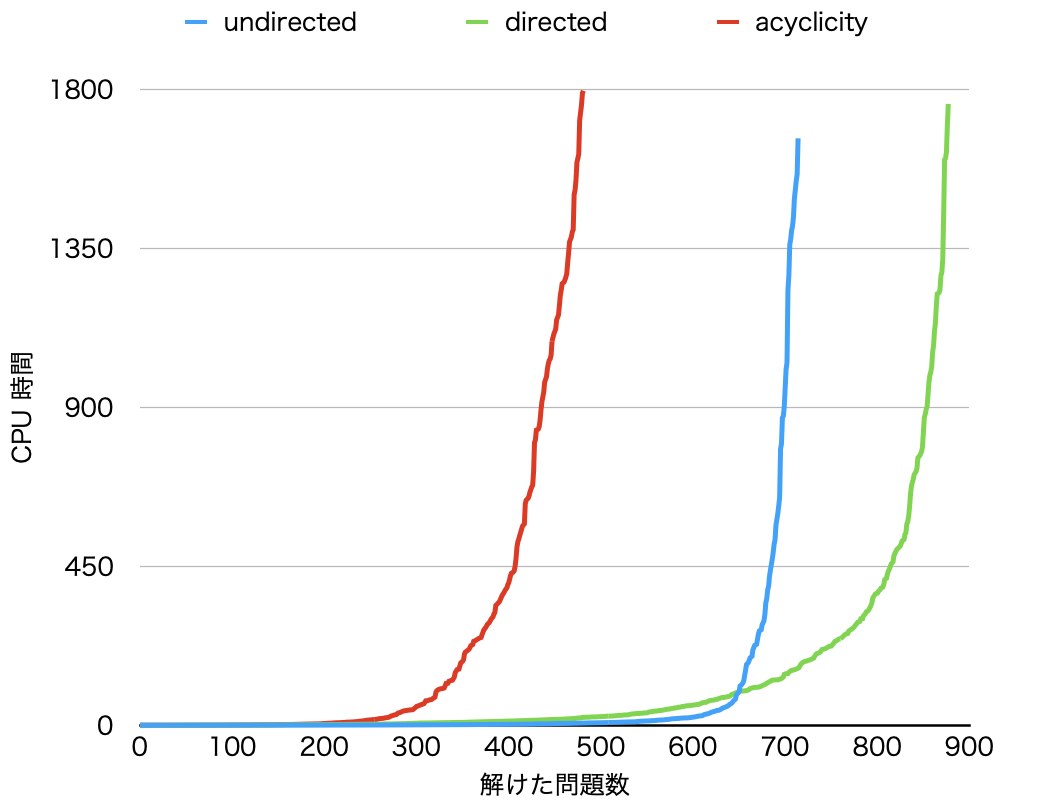
\includegraphics[width=0.7\linewidth]{fig/cactus.png}
\end{center}

\begin{itemize}
\item \code{directed} 符号化が,他の2つの符号化と比較して,
  より多くの問題を高速に解いていることがわかる.
\end{itemize}
\end{frame}

%%%%%%%%%%%%%%%%%%%%%%%%%%%%%%%%%%%%%%%%%%%%%%%%%%%%%%%%%%%%%%%%%%% 
\begin{frame}[shrink]{HCP: 解けた問題数の内訳}
%%%%%%%%%%%%%%%%%%%%%%%%%%%%%%%%%%%%%%%%%%%%%%%%%%%%%%%%%%%%%%%%%%% 
  
%%%%%%%%%%%%%%%%%%%%%%%%%%%%%%
\begin{center}
\scalebox{0.5}[0.5]{%\begin{tikzpicture}

%\end{tikzpicture}
}
% 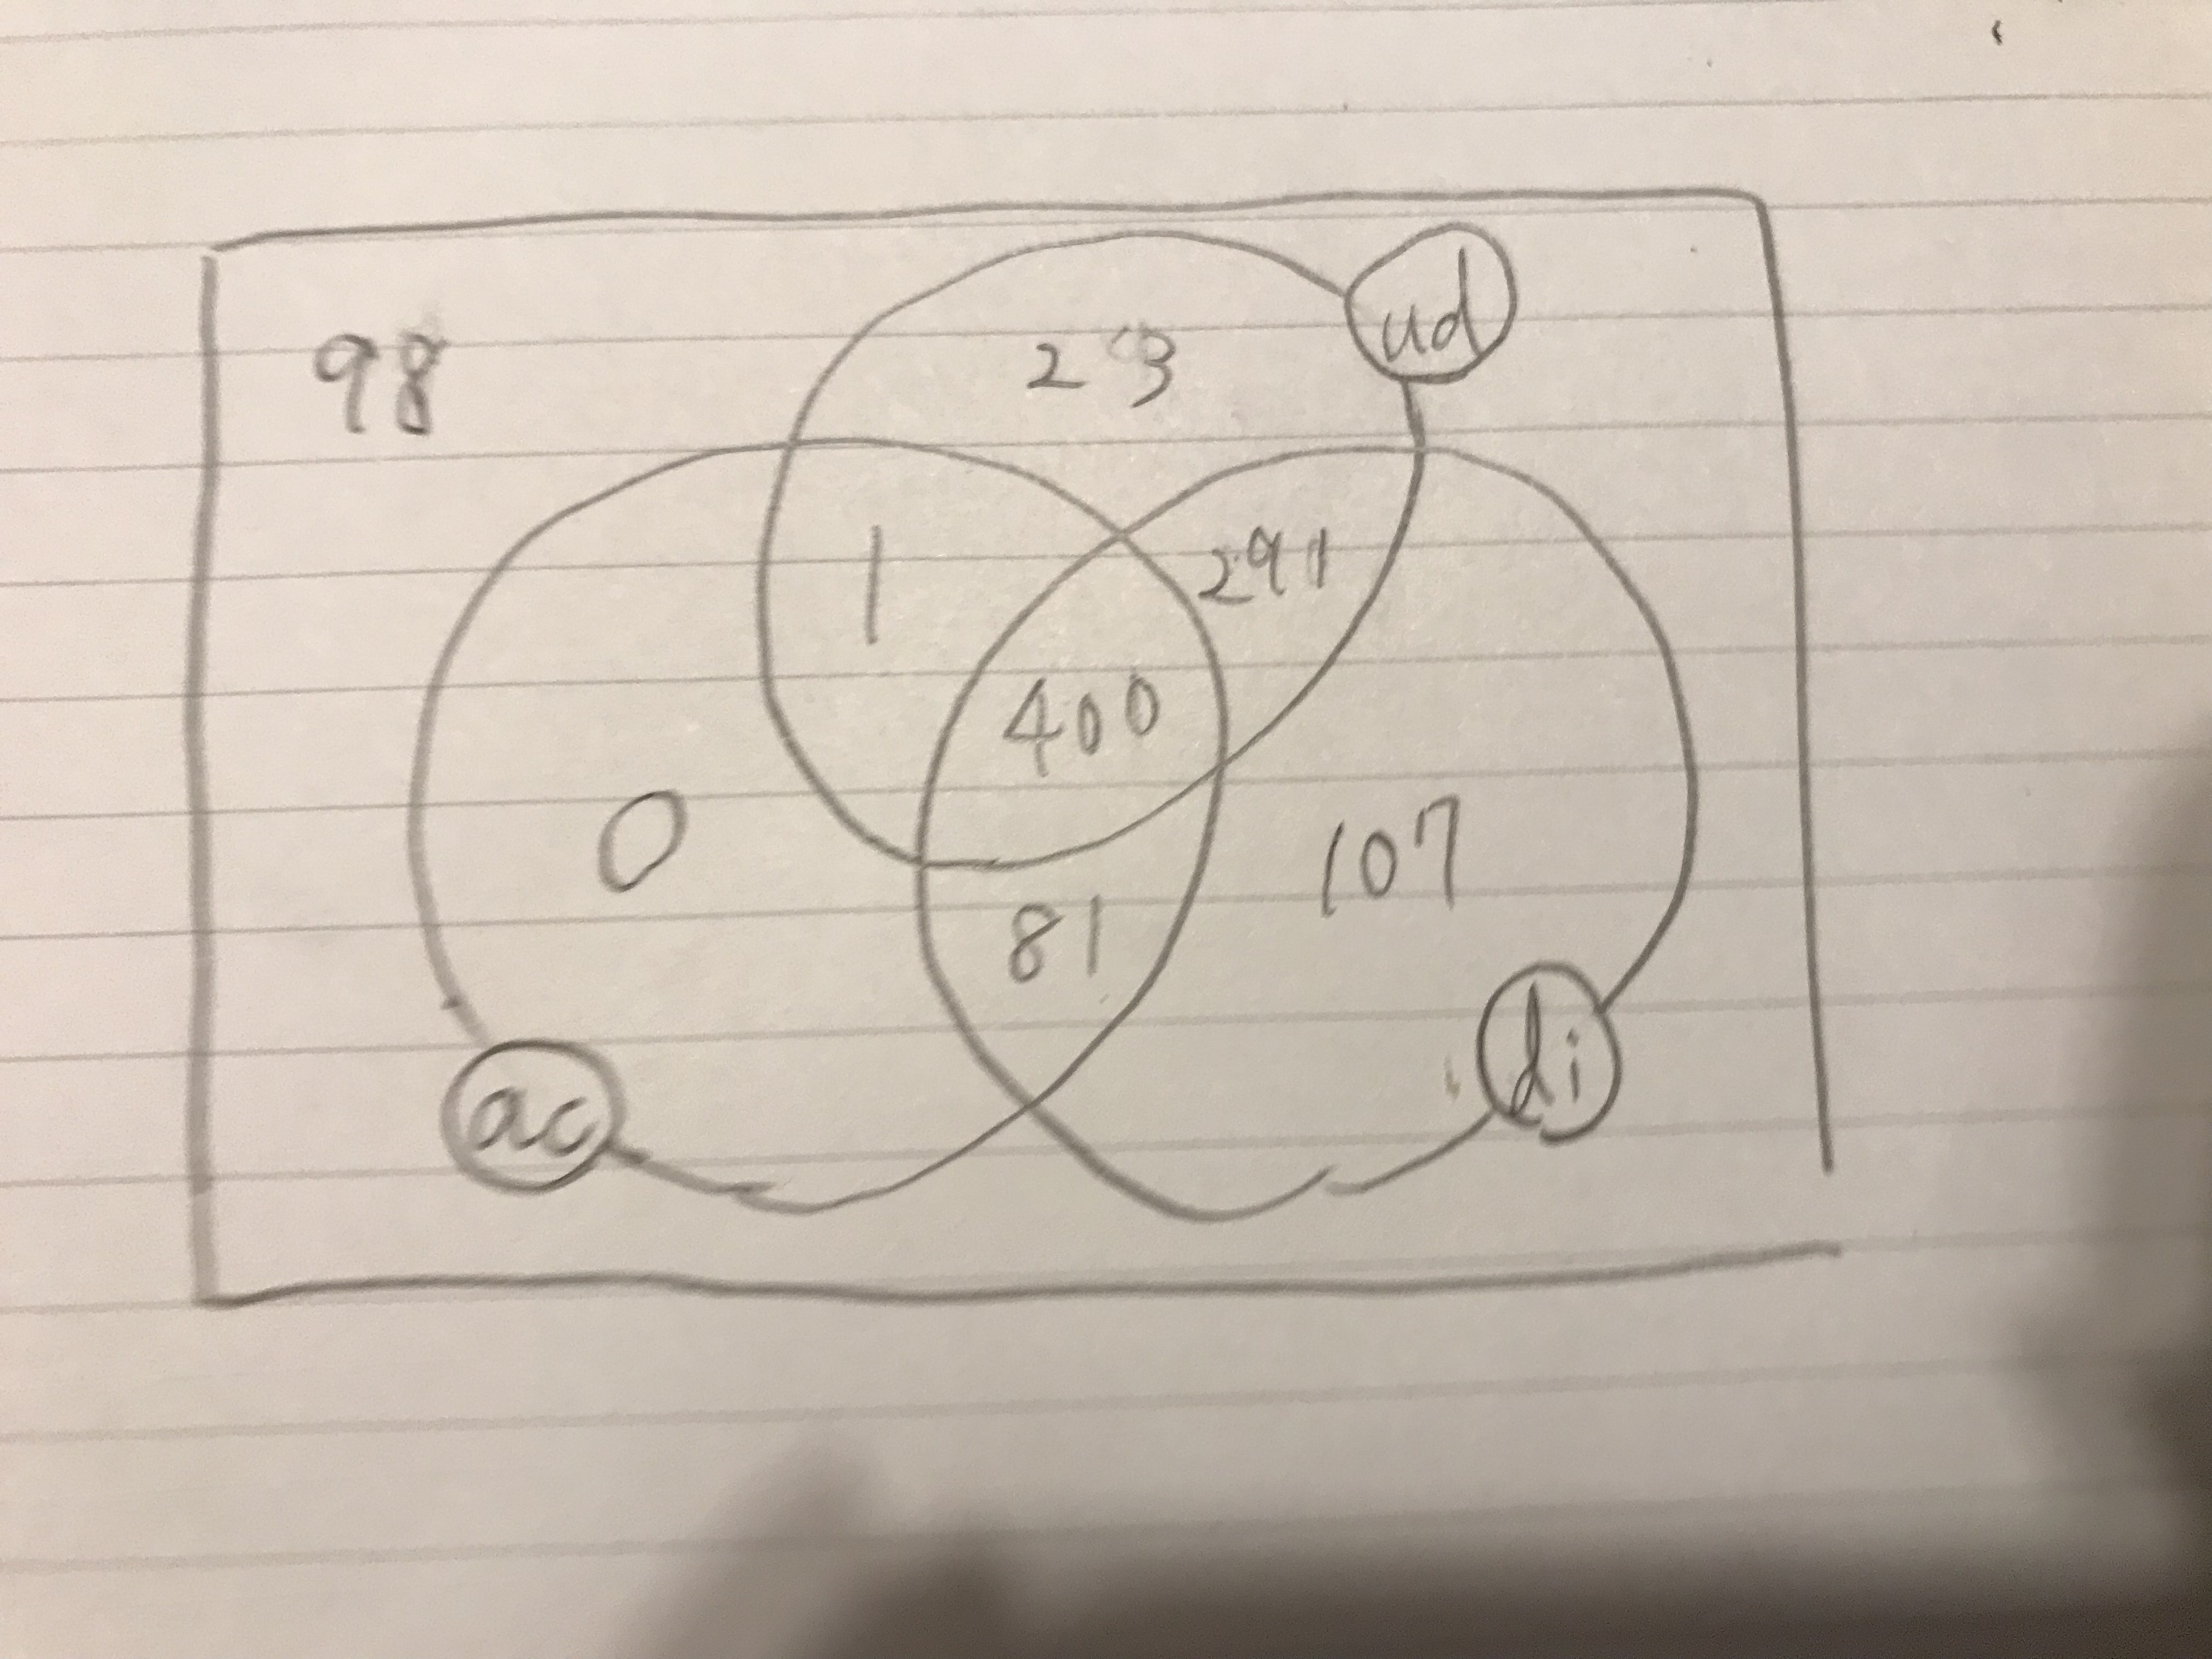
\includegraphics[width=0.5\linewidth]{fig/venn.jpeg}
\end{center}
%%%%%%%%%%%%%%%%%%%%%%%%%%%%%%
\vfill
\begin{itemize}
\item 全1,001問のうち,いずれかの符号化で解けた問題数は903問,
  どの符号化でも解けなかった問題数は98問であった.
\item \code{acyclicity} 符号化で解けた482問は,1問を除いて,
  \code{directed} 符号化でも解けている.
\item \code{undirected} と \code{directed} を比較すると,
  片方で解けて,もう片方で解けていない問題が一定数存在する.
\end{itemize}
\end{frame}

%%%%%%%%%%%%%%%%%%%%%%%%%%%%%%%%%%%%%%%%%%%%%%%%%%%%%%%%%%%%%%%%%%%
\begin{frame}{他のアプローチとの比較}
%%%%%%%%%%%%%%%%%%%%%%%%%%%%%%%%%%%%%%%%%%%%%%%%%%%%%%%%%%%%%%%%%%%
\begin{block}{}\centering
  FHCP Challenge 競技会(2015--2016)の上位5チームの成績~\footnotemark[3].
\end{block}
\vfill
\begin{tabular}[t]{clrc}
順位 & チーム & 問題数 & 手法 \\\hline
1 & INRIA, France & 985 & CPLEX \\
%\only<2>{ & \alert{ASP バーチャルベスト} & 903 & ASP \\}
\only<2>{ & \alert{ASP \code{directed} 符号化 (提案)} & 879 & ASP \\}
2 & IBM, United Kingdom & 614 & SAT \\
3 & King Saud University, Saudi Arabia & 488 & 不明 \\
4 & TU Darmstadt, Germany & 464 & 不明 \\
5 & Independent Researcher & 385 & 不明 \\\hline
\end{tabular}
\vfill

\begin{alertblock}<2>{}\centering
  提案手法は,ルール7個のASP符号化と汎用ソルバーの組合せで,
  \alert{実質2位に相当する成績}を示した.
\end{alertblock}

\footnotetext[3]{http://fhcp.edu.au/fhcpcs}
\end{frame}

%%%%%%%%%%%%%%%%%%%%%%%%%%%%%%%%%%%%%%%%%%%%%%%%%%%%%%%%%%%%%%%%%%%
\begin{frame}{まとめと今後の課題}
%%%%%%%%%%%%%%%%%%%%%%%%%%%%%%%%%%%%%%%%%%%%%%%%%%%%%%%%%%%%%%%%%%%
% \begin{alertblock}{}\centering
% ASP を用いたハミルトン閉路問題の解法について述べた.
% \end{alertblock}
% \vfill

\begin{enumerate}
\item \structure{HCP を解く3種類の ASP 符号化の実装(卒業研究)}
  \begin{itemize}
  \item ASP の \alert{ルール7個}程度で簡潔に表現できることを確認.
  \end{itemize}
\item \structure{\bf FHCPベンチマーク問題集を用いた評価実験}
  \begin{itemize}
  \item \code{directed} 符号化が879問と最も多くの問題を解き,
    他の符号化と比較して,その優位性が確認できた.
  \item FHCP Challenge 競技会の上位ソルバーの成績と比較した結果,
    directed 符号化は\alert{実質2位}に相当する性能を示した.
  \end{itemize}
\item \structure{\bf マルチショットASP解法を用いた手法の考案} (今回は省略)
\end{enumerate}

\begin{block}{今後の課題}
  \begin{itemize}
  \item マルチショットASP解法を用いた手法の改良
    \begin{itemize}
    \item Residue Number System を用いた
      HCP の ASP 符号化
    \end{itemize}
  \item 巡回セールスマン問題への拡張.
  \end{itemize}
\end{block}
\end{frame}

%%%%%%%%%%%%%%%%%%%%%%%%%%%%%%%%%%%%%%%%%%%%%%%%%%%%%%%%%%%%%%%%%%%
\begin{frame}{研究発表業績}
%%%%%%%%%%%%%%%%%%%%%%%%%%%%%%%%%%%%%%%%%%%%%%%%%%%%%%%%%%%%%%%%%%%
  \begin{enumerate}
  \item 平手貴大,宋剛秀,田村直之,番原睦則.
    解集合プログラミングを用いたハミルトン閉路問題の解法に関する考察.
    日本ソフトウェア科学会第38回大会講演論文集,34-L,2021年9月2日.
  \end{enumerate}
\end{frame}

%%%%%%%%%%%%%%%%%%%%%%%%%%%%%%%%%%%%%%%%%%%%%%%%%%%%%%%%%%%%%%%%%%%
%Appendix
\begin{frame}[noframenumbering]{}
 \thispagestyle{empty}
 \Huge 付録
\end{frame}
%%%%%%%%%%%%%%%%%%%%%%%%%%%%%%%%%%%%%%%%%%%%%%%%%%%%%%%%%%%%%%%%%%%
\begin{frame}[noframenumbering]{コスト制約付きハミルトン路問題}
%%%%%%%%%%%%%%%%%%%%%%%%%%%%%%%%%%%%%%%%%%%%%%%%%%%%%%%%%%%%%%%%%%%
\thispagestyle{empty}
\begin{center}
  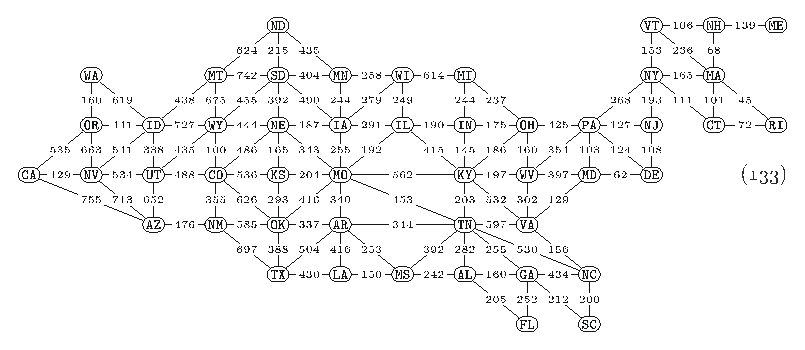
\includegraphics[width=0.8\linewidth]{fig/taocp_vol4fasc1b_p52_eq133.pdf}
\end{center}
\vfill
\only<1>{
\begin{itemize}
\item Knuth の The Art of Computer Programming に記載されている米国本
  土48州の隣接関係を表すグラフ
\item 頂点数は48,辺の数は105
\item 各辺に付与されている数字は州都の間の距離 (マイル)
\end{itemize}
}
\only<2>{
\begin{exampleblock}{}
  西海岸ワシントン州 (WA) から 東海岸メーン州 (ME) までの距離の総和
  がある閾値以下であるハミルトン路を求める問題を考える.
\end{exampleblock}
\begin{itemize}
\item WA から ME までのハミルトン路は 6,876,928 通りあり,
  最短ハミルトン路は 11,698 マイルである.
\item 閾値を最短距離の 10\%増 (12,868 マイル) とした場合,
  解の総数は 16,180 個ある.
\end{itemize}
}
\end{frame}

%%%%%%%%%%%%%%%%%%%%%%%%%%%%%%%%%%%%%%%%%%%%%%%%%%%%%%%%%%%%%%%%%%%
\begin{frame}[noframenumbering]{HCP: 解けた問題数}
%%%%%%%%%%%%%%%%%%%%%%%%%%%%%%%%%%%%%%%%%%%%%%%%%%%%%%%%%%%%%%%%%%%
\thispagestyle{empty}
%%%%%%%%%%
\begin{table}[t]\scriptsize
  \centering
  %\tabcolsep = 0.8mm
  \renewcommand{\arraystretch}{1.2}
  \begin{tabular}{lr|rrr}
    問題サイズ & 問題数 & \textsf{undirected} & \textsf{directed} & \textsf{acyclicity}\\
   \hline
    $\:\:\:\:\:\,\, 0 \leq |V| < 1000$     & 171   & 156   & \alert{171}   & 156  \\ %
    $1000 \leq |V| < 2000$  & 165   & 120   & \alert{159}   & 121  \\
    $2000 \leq |V| < 3000$  & 177   & 125   & \alert{163}   & 80   \\
    $3000 \leq |V| < 4000$  & 185   & 104   & \alert{147}   & 48   \\
    $4000 \leq |V| < 5000$  & 128   & 92    & \alert{106}   & 30   \\
    $5000 \leq |V| < 6000$  & 80    & 63    & \alert{70}    & 21   \\
    $6000 \leq |V| < 7000$  & 55    & 39    & \alert{41}    & 20   \\
    $7000 \leq |V| < 8000$  & 28    & 12    & \alert{15}    & 4    \\
    $8000 \leq |V| < 9000$  & 10    & 2     & \alert{5}     & 1    \\
    $9000 \leq |V| < 10000$  & 2     & \alert{2}     & \alert{2}     & 1    \\
   \hline
    合計 & 1001 & 715   & \alert{879}   & 482  
  \end{tabular}
  \vskip .5em
%  \caption{ハミルトン閉路問題: 解けた問題数}
  \label{sat_table}
\end{table}
%label{sat_table}
%%%%%%%%%%

\begin{itemize}
\item \code{directed} 符号化が最も多い 879 問を解いた.
\item \code{directed} 符号化は,どの頂点数の範囲においても良い結果を示
  しており,その優位性が確認できる.
\end{itemize}
\end{frame}

%%%%%%%%%%%%%%%%%%%%%%%%%%%%%%%%%%%%%%%%%%%%%%%%%%%%%%%%%%%%%%%%%%%

\end{document}

%%% Local Variables:
%%% mode: japanese-latex
%%% TeX-master: t
%%% End:
